%%
%% 研究報告用スイッチ
%% [techrep]
%%
%% 欧文表記無しのスイッチ(etitle,eabstractは任意)
%% [noauthor]
%%

%\documentclass[submit,techrep]{ipsj}
\documentclass[submit,techrep,noauthor]{ipsj}
\usepackage[dvips,dvipdfmx]{graphicx}
\usepackage{latexsym}
\usepackage{comment}
\usepackage{here}
\usepackage{cite}
\usepackage{url}
% added by iguchi_t below.
\usepackage{listings}
\usepackage{multirow} % multirow 環境を使おうとすると何故か citation がうまく表示されなくなる

% 囲み枠
\usepackage{ascmac,fancybox,txfonts}
\usepackage{caption}

% float 環境関連(図表)
\usepackage{float}
\usepackage{longtable,booktabs}
\usepackage{tabularx}

\lstset{%
    numbers=left,
    breaklines=true,
    frame=shadowbox,
    basicstyle={\ttfamily\small},
    numberstyle={\scriptsize},
    lineskip=-0.5ex
}

% end here.

\def\Underline{\setbox0\hbox\bgroup\let\\\endUnderline}
\def\endUnderline{\vphantom{y}\egroup\smash{\underline{\box0}}\\}
\def\|{\verb|}
%

%\setcounter{巻数}{59}%vol59=2018
%\setcounter{号数}{10}
%\setcounter{page}{1}

\renewcommand{\lstlistingname}{コード}

\def\sysname{VampOS}
\def\Sysname{VampOS}

\def\rr{Reboot-based Recovery}

% \def\rh{per-object recovery handler}
% \def\Rh{Per-object recovery handler}

% \def\rhs{per-object recovery handlers}
% \def\Rhs{Per-object recovery handlers}

% \def\mlist{M-list}
% \def\Mlist{M-List}

% \def\nmiq{NMI shepherd}
% \def\Nmiq{NMI shepherd}

% \def\ptdup{PTDUP}
% \def\Ptdup{PTDUP}

\begin{document}

\title{Reboot-based Recovery を指向する Unikernel}
%\etitle{A Recovery Mechanism for the Kernel-level ECC-uncorrectable Error}

\affiliate{tuat}{東京農工大学\\
Tokyo University of Agriculture and Technology}

\author{和田 健}{Takeru Wada}{tuat}
\author{山田 浩史}{Hiroshi Yamada}{tuat}

\begin{abstract}
Reboot-based Recovery は,ソフトウェアの再起動によって,
コンピュータシステムをフォールトや不安定な状態からリカバリするためのシンプルかつ強力な方法である.
\rr は,\emph{Unikernel} と呼ばれる新しいタイプのオペレーティングシステムへの適用という課題に直面している.
Unikernel は,OS の機能がライブラリのようにアプリケーションにリンクするライブラリ OS である.
アプリケーションと Unikernel が密接に結びつくために,Unikernel のみの再起動にアプリケーションの再起動を伴うことになり,
Unikernel に関係のないメモリの内容を消去し,再構築してしまう.
本論文では,Unikernel のみの \rr を効率的に行う \emph{VampOS} を紹介する.
VampOS は,Unikernel コンポーネント間のインタラクションを記録し,
再起動したコンポーネントにそれらを再実行させることで,
リンクされたアプリケーションの実行状態を維持したまま,
Unikernel のコンポーネント単位での Reboot-based Recovery を行う.
Reboot-based Recovery の前段階であるソフトウェア若化を
行う最適化されていない VampOS のプロトタイプを Unikraft 0.8.0 に実装した.
プロトタイプを用いた実験により,
実行時のオーバヘッドは最大で 13.6 倍であることと,
意図的に挿入したメモリリークのバグの影響を僅かなダウンタイムで緩和することを示した.
また,本論文では,Unikernel の効率的な Reboot-based Recovery の実現のための
次の方向性について述べる.

\end{abstract}

\begin{jkeyword}
    Reboot-based Recovery, ソフトウェア若化,Unikernels
\end{jkeyword}

% Software rejuvenation is a simple but powerful
% method for improving the availability of computer systems.
% Software rejuvenation faces a challenge to apply itself to a new
% type of application, the Unikernel which is a library OS where
% OS functions are linked to the target applications like libraries.
% Since the unikernel layer is tightly coupled to applications,
% rebooting the unikernel layers involves the applications’ reboots,
% eliminating and reconstructing memory contents unrelated to the
% unikernels. This paper presents VampOS that allows us to rejuve-
% nate the only unikernel layer. VampOS performs component-level
% rejuvenation of the unikernel by logging interactions between
% the components and replaying them to restarted components
% while simultaneously keeping the linked applications running.
% We implemented a prototype of VampOS, not well-optimized, on
% Unikraft 0.8.0 and the experimental results show that its runtime
% overhead is up to 13.6× and the VampOS-linked SQLite mitigates
% the effects of the intentionally injected memory leak bugs without
% any downtime. This paper also describes the next directions for
% efficient rejuvenation of the unikernel-linked applications.




\maketitle

\section{はじめに} \label{section:introduction}

\rr は,ソフトウェアを故障や不安定な状態からリカバリするためのシンプルかつ強力な方法であり,
アプリケーションを再起動することで,その実行状態をリフレッシュする.
定期的なアプリケーションの再起動は,\emph{ソフトウェア若化}と呼ばれ,
解放忘れのメモリオブジェクトや閉じ忘れたディスクリプタなどの古くなったり漏れたりしているリソースを回収することで,
アプリケーションのクラッシュを未然に防ぐことができる.
ソフトウェア若化は,故障の根本的な原因を解析することなしに故障からリカバリすることができるうえ,
アプリケーションの修正をせずに適用できるため,
エンドユーザにとってのソフトウェアのエラーや不具合への唯一の対策となることがしばしばある.
また,\rr は,クラッシュやハングアップからアプリケーションをリカバリするためにも使われる.
その有用性から \rr の適用範囲を拡大するために,
研究者たちは Java アプリケーション~\cite{CandeaEtAl-Microreboot}やインメモリデータベース~\cite{JumonjiEtAl-WoSAR17,JumonjiEtAl-IEICE2021},
オペレーティングシステム~\cite{YamakitaEtAl-PBR,DepoutovitchEtAl-otherworld,KouraiEtAl-cachemind,TeradaEtAl-Dwarf,BovenziEtAl-ISSRE13},
ハイパーバイザ~\cite{KouraiEtAl-Roothammer,KouraiEtAl-TDSC,LeEtAl-VEE11}などの様々なソフトウェアレイヤに対して有効なソフトウェアメカニズムを提案している.

\rr は,\emph{Unikernel} と呼ばれる新しいタイプのオペレーティングシステムへの適用にするという課題に直面している,
Unikernel ~\cite{MadhavapeddyEtAl-Unikernel,KivityEtAl-OSv,SartakovEtAl-ASPLOS21,KanteeEtAl-rumprun,KuenzerEtAl-Unikraft}は,
OS の機能がライブラリのようにアプリケーションにリンクするライブラリ OS であり,
特にクラウド環境において利点となるいくつかのメリットを提供する.
第一に,Unikernel は,アプリケーションと同じ保護モードで動作するため,
システムコールを実行時にモード切り替えが発生せず,
システムコールオーバヘッドの問題が軽減される.
第二に,
すべての機能を内包する
汎用的に使われるモノリシック OS カーネルとは異なり,
Unikernel では,
アプリケーションの実行に必要な OS コンポーネントのみをリンクするため,
Unikernel にリンクされたアプリケーションのメモリフットプリントが小さい.
第三に,
不必要な OS コンポーネントを排除することで,
Unikernel にリンクされたアプリケーションのトラステッドコンピューティングベース(TCB)を小さく保ち,
攻撃の標的となるものを減らすことができる.

Unikernel の主要なタスクは,ハイパーバイザ上でリンクされたアプリケーションの実行を制御することであるため,
できるだけ信頼性を高いものにしたほうが良く,Unikernel レイヤのみの \rr は有用である.
例えば,Unikernel が経年劣化によって停止したときに,
Unikernel にリンクされたアプリケーションは正常に動作しなくなる.
しかし,Unikernel レイヤのみの \rr を効率的に行うことは困難である.
Unikernel レイヤとアプリケーションの結びつきが強いため,
アプリケーションの再起動を伴うことになり,
Unikernel に関係のないメモリの内容を消去し,再構築してしまう.
実行中のアプリケーションの再起動を伴わない OS カーネルのみを若返らせるソフトウェアメカニズム~\cite{DepoutovitchEtAl-otherworld,TeradaEtAl-Dwarf}が提案されているものの,
それらの設計はモノリシック OS カーネルが対象であり,
アプリケーションの実行ごとに OS コンポーネントが異なる Unikernel には適さない.

汎用 OS と比較して,Unikernel が限定的な機能しか持たないとはいえ,Unikernel がソフトウェアバグを含まないわけではない.
実際に,現在進行中の Unikernel のプロジェクトにはいくつものバグが報告されている~\cite{Issues-Unikraft,Issues-OSv,Issues-Mirage}.
報告されているものの中には,経年劣化に関連するバグも存在する~\cite{Unikraft-memleak,Mirage-memleak}.
また,アプリケーションに必要な機能を提供するために,
アプリケーションの要件に合わせて
サードパーティ製のライブラリを組み合わせた構成にカスタマイズすることもある.


本論文では,
効率的に Unikernel レイヤのみの \rr を実現する \emph{\sysname} を紹介する.
VampOS は,
リンクされたアプリケーションの実行状態を維持したまま,
Unikernel のコンポーネント単位での Reboot-based Recovery を行う.
VampOS は,Unikernel のカスタマイズ性を利用する.
Unikernel のコンポーネントは互いに高度に独立し,
コンポーネント間のインタフェースは明確に定義されている.
\sysname は,対象のコンポーネントを再起動し,
再起動したコンポーネントに
コンポーネント間のインタラクションを記録したもの
を再実行させることで,
コンポーネントの実行状態をリフレッシュしたメモリの内容とともに復元する.

Reboot-based Recovery の前段階であるソフトウェア若化を
行う VampOS のプロトタイプ Unikraft 0.8.0 に実装し,
VampOS の有効性を示す予備実験を行った.
実験の結果は,その実行時のオーバヘッドは最大で 13.60 倍であるものの,
VampOS にリンクされたリレーショナルデータベースである SQLite に
意図的に挿入したメモリリークのバグの影響を僅かなダウンタイムで緩和することを確認した.
本研究は,Unikernel の効率的な \rr を実現するための最初の段階であり,
プロトタイプは十分に最適化されていない.
しかし,Unikernel にリンクされたアプリケーションの効率的な \rr のための次の方向性を明確に捉えることができた.

本論文の構成は次のとおりである.
第 2 章では本研究の背景について述べ,
第 3 章では VampOS の全体像を示す.
第 4 章では,VampOS のプロトタイプを用いた予備実験とその結果について述べる.
第 5 章では,本研究の現状と次の方向性について述べる.

% % rejuvenation
% Software rejuvenation~\cite{HuangEtAl-rejuvenation,CotroneoEtAl-rejuvenation-survey,CotroneoEtAl-Surv14} is a simple but powerful method for improving the availability of computer systems. Software rejuvenation refreshes the running states of an application by restarting it. Periodically performing software rejuvenation reclaims stale or leaked resources as memory leaks and descriptor leaks, a.k.a. \emph{software aging}, resulting in preventing application crashes. Software rejuvenation allows us to recover from failures without analyzing their root causes. In addition, this method is applicable to ``as-is'' applications and thus often becomes the only remedy against software errors and failures for end users. To extend the applicability of software rejuvenation due to its usefulness, researchers have proposed effective software mechanisms for various software layers such as java applications~\cite{CandeaEtAl-Microreboot}, in-memory databases~\cite{JumonjiEtAl-WoSAR17,JumonjiEtAl-IEICE2021}, operating systems (OSes)~\cite{YamakitaEtAl-PBR,DepoutovitchEtAl-otherworld,KouraiEtAl-cachemind,TeradaEtAl-Dwarf,BovenziEtAl-ISSRE13}, and hypervisors~\cite{KouraiEtAl-Roothammer,KouraiEtAl-TDSC,LeEtAl-VEE11}.

% % unikernel
% Software rejuvenation faces a challenge in applying itself to a new type of applications, \emph{Unikernels}. The unikernel~\cite{MadhavapeddyEtAl-Unikernel,KivityEtAl-OSv,SartakovEtAl-ASPLOS21,KanteeEtAl-rumprun,KuenzerEtAl-Unikraft} is a library OS where OS functions are linked to the target applications like libraries. It offers several benefits that are advantages, especially in cloud environments. First, the overhead of system call issues is mitigated since the unikernel runs on the same protection mode as the applications, and thus the system calls do not cause mode changes. Second, the memory footprint of the unikernel-linked applications is small since the applications can link only OS components required for their execution, different from widely-used monolithic OS kernels that contain full OS functionalities. Third, we can keep the trusted computing base (TCB) of the unikernel-linked applications small by removing unnecessary OS components, thus reducing attack surfaces.

% % what's challenge
% Rejuvenating the unikernel layer is helpful since it is better to make the unikernel layer as reliable as possible due to its primary task of controlling linked application execution on top of the hypervisor. For example, the applications cannot run correctly when unikernels are down by aging-related bugs. However, efficient rejuvenation of unikernels does not come for free. Since the unikernel layer is tightly coupled to applications, rebooting the unikernel layers involves the applications' reboots, eliminating and reconstructing memory contents unrelated to the unikernels. Although software mechanisms~\cite{DepoutovitchEtAl-otherworld,TeradaEtAl-Dwarf} for rejuvenating the OS kernels without restarting the running applications have been proposed, the implicit assumption of their designs is that the target OS kernels are monolithic; they are not suitable for unikernels whose runtime components are different among applications.

% This paper presents \emph{\sysname}, which achieves efficient software rejuvenation of the unikernel layer. {\sysname} allows us to perform component-level rejuvenation of the unikernel while simultaneously keeping the linked applications running. The key behind {\sysname} is to exploit unikernels' customizability; the components are highly independent of each other and interfaces between each component are well defined. {\sysname} restarts the target components and restores the running states with flesh memory contents by logging interactions between them and replaying them to the restarted components.

% We prototyped {\sysname} on Unikraft {\version} and conducted some preliminary experiments to show the effectiveness of {\sysname}. The experimental results show that its runtime overhead is up to 13.60{\texttimes} and the {\sysname}-linked SQLite, which is a widely-used relational database, mitigates the effects of the intentionally injected memory leak bugs without any downtime. This work is the first-step to making unikernels rejuvenatable, and the prototype has not been well-optimized yet. Through this work, we clearly capture the next directions for efficient rejuvenation of the unikernel-linked applications. 

% The rest of the paper is organized as follows. Sec.~\ref{sec:bg} introduces the background of this work and Sec.~\ref{sec:prop} shows an overview of {\sysname}. Sec.~\ref{sec:design} describes the design details of {\sysname} and Sec.~\ref{sec:exp} conducts preliminary experiments with a prototype of {\sysname} and their results. Sec.~\ref{sec:next} finally mentions the current status of the work and the next directions. 



\section{背景} \label{sec:background}


\subsection{Unikernels}

Unikernel は,対象のアプリケーションにリンクし,
アプリケーションと同じ保護モードからのハイパーコールを介して,
下層のハイパーバイザに計算資源を要求する.
Unikernel はリンクされたアプリケーションとアドレス空間を共有するため,
一般的な Unikernel は,マルチプロセスアプリケーションではなく,
シングルプロセスで動作するアプリケーションのみをサポートする.
Unikernel は,特にクラウド環境で受け入れられている.
クラウド環境上の個々の仮想マシン (VM) は通常,
1 つのアプリケーションのみを実行するため,
OS の機能の一部のみを使用するためである.
研究者たちは,セキュリティアーキテクチャ~\cite{MadhavapeddyEtAl-Unikernel}や
様々なアプリケーションへのサポート~\cite{KivityEtAl-OSv,ZhangEtAl-Kylinx,WilliamsEtAl-SoCC18,OlivierEtAl-VEE19},
組み込みクラウド用のマルチテナントコントローラ~\cite{MadhavepeddyEtAl-Jitsu},
軽量ネットワーク機能の仮想化~\cite{MartinsEtAl-NSDI14},
軽量特権仮想マシン~\cite{MehrabEtAl-Kite},
モジュラリティの向上~\cite{KuenzerEtAl-Unikraft,KuenzerEtAl-SYSTOR19},
コンポーネント間のアイソレーションの強化~\cite{LefeuvreEtAl-FlexOS,SartakovEtAl-ASPLOS21}
を含む Unikernel の仕組みと適用範囲を研究している.

\begin{figure}[t]
    \begin{center}
      \begin{tabular}{c}
        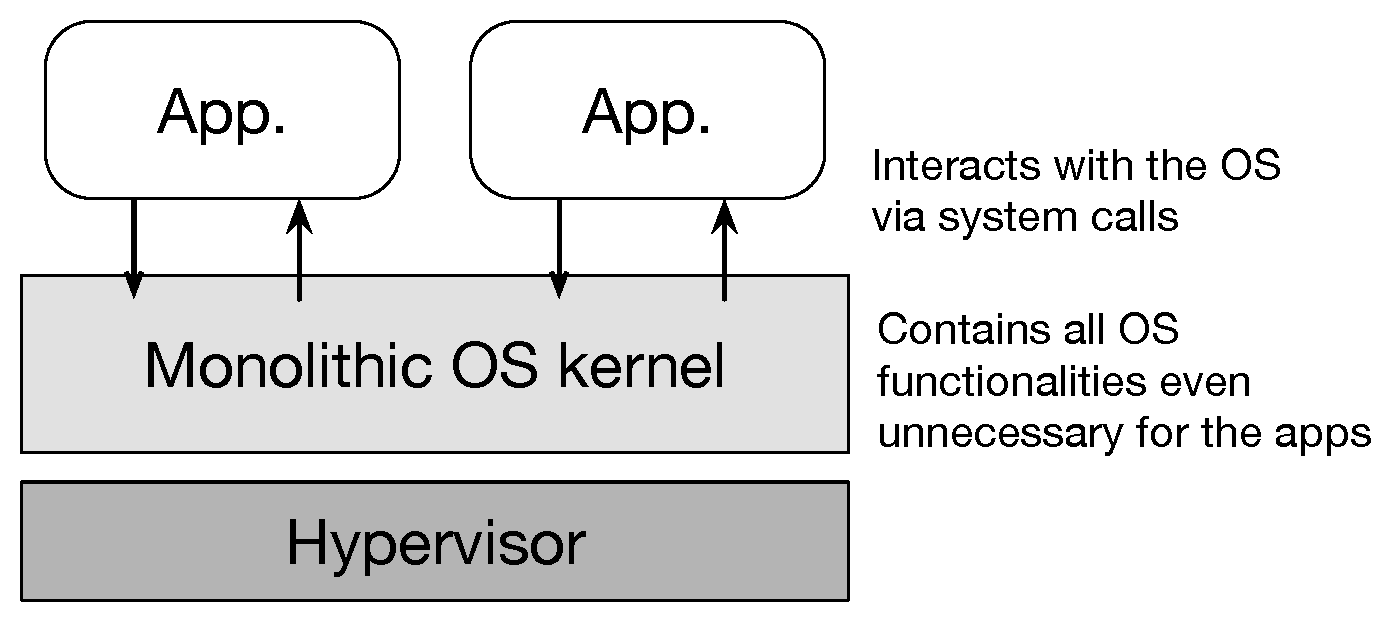
\includegraphics[scale=0.3]{./img/monolithic.eps} \\
        (a) Conventional Monolithic OS kernel       \vspace*{2mm} \\ 
        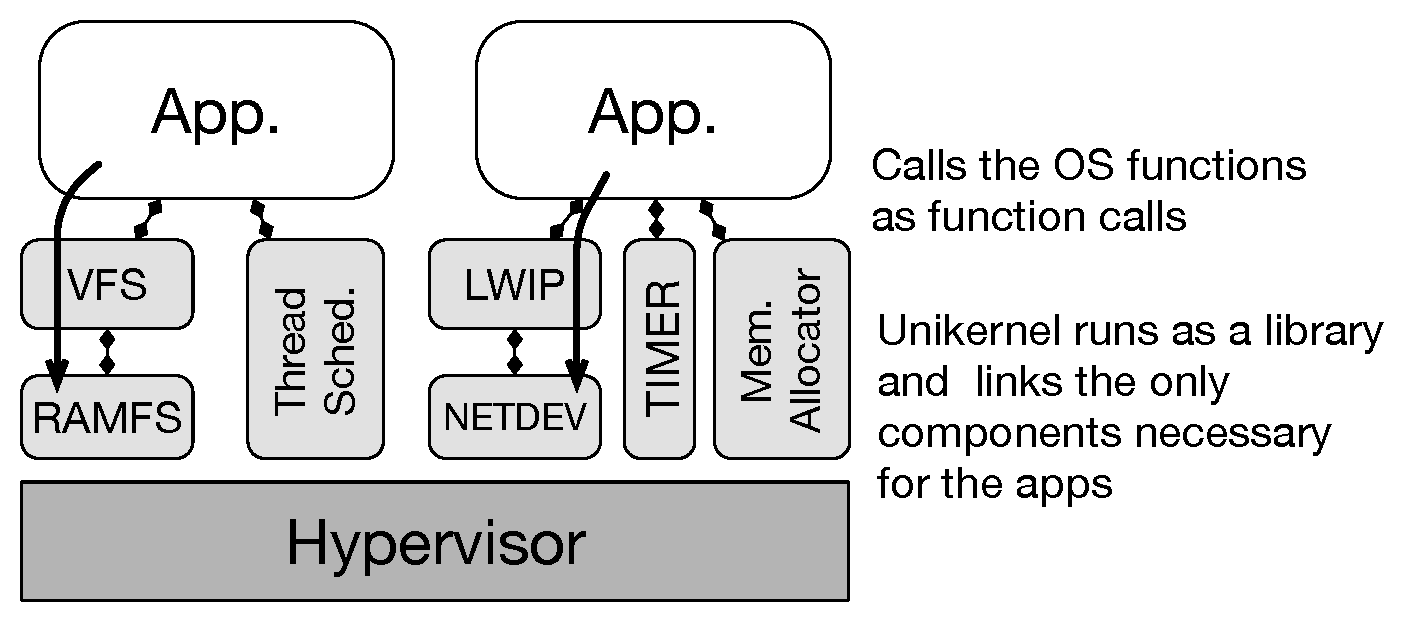
\includegraphics[scale=0.3]{./img/unikernel.eps} \\
        (b) Unikernel \\
      \end{tabular}
      \caption{\textbf{OS カーネルアーキテクチャの違い} \textit{従来の OS カーネルは,アプリケーションと対話するためのシステムコールを公開し,実行中のアプリケーションに不必要な OS 機能さえもすべて含んでいる.Unikernel はライブラリとして動作し,アプリケーションが動作するのに必要なコンポーネントのみをリンクする.}}
      \label{fig:kernels}
    \end{center}
  \end{figure}

図\ref{fig:kernels}は,従来のモノリシックカーネルと Unikernel の違いを示している.
Linux のような従来の OS カーネルでは,ファイルシステムやネットワークスタックのようなすべてのサブシステムをその必要性に関係なく含んでおり,
アプリケーションより高い特権レベルで動作する.
アプリケーションは計算資源を要求するためにシステムコールを発行し,
トラップすることによって,下層の OS カーネルに特権操作を行う.
一方で,Unikernel は対象のアプリケーションに直接リンクし,
同じアドレス空間で同じ特権モードで動作する.
アプリケーションは,
動作に必要な OS コンポーネントのみを選択して,リンクすることができる.
これらの特徴は,従来の OS カーネルと比較して,
高速なシステムコール発行やブート時間の短縮,
メモリフットプリントの縮小,OS カーネルレイヤのコードサイズの縮小を含む
いくつかの利点を提供する.

本論文では,
\emph{どのように Unikernel の効率的な \rr を実現するのか?}
という問いについて答えようとするものである.
Unikernel レイヤの信頼性をできるだけ高いものにしたほうが良い.
Unikernel はアプリケーションとハイパーバイザの中間に位置し,
計算資源をハイパーバイザに要求し,
リンクしたアプリケーションにその計算資源を与えるので,
Unikernel レイヤに障害が発生すると
アプリケーションは実行状態を維持することができなくなる.
OS カーネルは,その複雑性と変化し続ける機能から,
過去数十年に渡る多くの努力~\cite{ChouEtAl-SOSP01,PalixEtAl-ASPLOS11,Syzkaller,PanEtAl-SEC17,PailoorEtAl-SEC18,SchumiloEtAl-kAFL, TalebiEtAl-SEC21}
を以ってしてもバグのないソフトウェアからは程遠い.
そして,Unikernel を定期的に再起動し,
リフレッシュしたメモリの内容の使用を強制することは,
クラウドサービスを安定して提供するのに有効である.

しかし,効率的な Unikernel の \rr は容易ではない.
Unikernel がアプリケーションと密接に結びつくために,
Unikernel の再起動がアプリケーションの再起動を伴うことになり,
Unikernel に関係のないメモリの内容を消去し,再構築してしまう.
これは,
最近のインメモリデータベースやインメモリ分散フレームワークのようなインメモリアプリケーションにおいて重要なことである.
メモリフットプリントが数十 GB から数百 GB になり,
実行状態の復元に時間がかかるためである.
ある研究では,
Facebook のサーバを一度に 2 \% だけを再起動すると,
再起動時間は約 12 時間まで延長され,
ユーザはクエリの結果の一部しか見ることができないことが報告されている~\cite{GoelEtAl-SIGMOD14}.

\subsection{過去のアプローチ}

対象のソフトウェアを効率的に再起動するための
ソフトウェアメカニズムはこれまでにも模索されている.
いくつかの研究では OS カーネルの効率的な再起動に注目している.
KUP~\cite{KashyapEtAl-KUP}は,OS カーネルが再起動しても,アプリケーションの実行を維持する.
KUP は,メモリ上の対象のアプリケーションのユーザスペースのチェックポイントメカニズム~\cite{CRIU}を用いたスナップショットを取得し,
OS の再起動後にスナップショットを復元する.
このアプローチを Unikernel にリンクされたアプリケーションに適用することができない.
従来の OS カーネルとは異なり,
リンクされたアプリケーションと共有する単一のアドレス空間のみをサポートする Unikernel では,
チェックポイントの取得処理を対象のアプリケーションと同時に実行することができない.
また,
アプリケーションと Unikernel の境界が不明確であり,Unikernel のカスタマイズ性によりアプリケーションとは異なるため,
Unikernel にリンクされたアプリケーション以外が,対象のアプリケーションレイヤのみのスナップショットを取ることは困難である.


Otherworld~\cite{DepoutovitchEtAl-otherworld}や Dwarf~\cite{TeradaEtAl-Dwarf}は,
アプリケーションを動作させながら OS カーネルの再起動をする.
OS カーネルを再起動する際に,
Otherworld は新しいカーネルを起動し,
古い OS カーネルのメモリ上のプロセスコンテキストのカーネルメモリオブジェクトを強制的に回収し,
その内部構造を新しい OS カーネルに復元する.
Dwarf は,対象のアプリケーションに対するプロセスコンテキストのコアをハイパーバイザに保存し,
新しく起動した仮想マシン上に OS カーネルを起動し,
対象のアプリケーションを古い仮想マシンから新しい仮想マシンへと移行しながら,
新しいカーネルにアプリケーションの動作状態を強制的に復元させる.
これらのアプローチの前提として,対象の OS カーネルが\emph{モノリシック}であり,
Unikernel のコンポーネントがアプリケーションとは異なり,
プロセスコンテキストを維持するためのカーネルオブジェクトが一定ではないため,
Unikernel の特性に適したアプローチとはいえない.


Microreboot~\cite{CandeaEtAl-Microreboot}は,
細かい粒度でのソフトウェアの再起動を実現する.
Microreboot を可能にするために,
対象のアプリケーションは,
再起動の単位となる独立した小さいソフトウェアコンポーネントに分割される.
小さいコンポーネントの再起動が故障から回復できない場合には,
より大きいコンポーネントが再起動される.
このアプローチの暗黙の仮定として,
Microreboot される各コンポーネントは状態を持たないので,
対象のアプリケーションは,任意のコンポーネントの再起動に渡って,
一貫して動作し続ける.
Unikernel のコンポーネントは状態を持つことが多く,
ファイルシステムやネットワークのような状態を持つコンポーネントの再起動に渡って,
アプリケーションが一貫して動作し続けることは難しい.

Phase-baseds~\cite{YamakitaEtAl-PBR}や ShadowReboot~\cite{YamadaEtAl-ShadowR},CacheMind~\cite{KouraiEtAl-cachemind}を含む
効率的な OS の再起動に対するアプローチは,
OS カーネルの再起動によって引き起こされるダウンタイムとパフォーマンスの低下を軽減する.
通常の OS の再起動のように,これらのアプローチはすべての動作中のアプリケーションの再起動を伴い,
メモリフットプリントが大きなインメモリアプリケーションにおいて深刻なパフォーマンスの低下を引き起こす.
ハイパーバイザのソフトウェア若化をサポートするアプローチでは,
ハイパーバイザの再起動渡って,仮想マシンの動作状態を維持する.
これらのアプローチは,私たちのアプローチと補完関係にある.

いくつかのアプローチは Unikernel の信頼性の向上を目的としている.
Unikraftt~\cite{KuenzerEtAl-Unikraft}は,
Unikernel のモジュラリティを高め,
TCB をできるだけ小さくすることによってカスタマイズ性と信頼性を向上させている.
CubicleOS~\cite{SartakovEtAl-ASPLOS21}と FlexOS~\cite{LefeuvreEtAl-FlexOS}は,
故障したコンポーネントから他のコンポーネントへのエラー伝搬を防ぐために
Unikernel のコンポーネント同士を強く分離するものである.
これらのアプローチは,
Unikernel がリンクするアプリケーションの信頼性を維持するために,
私たちのアプローチとは補完的な立ち位置にある.
これらのアプローチでは,Unikernel が経年劣化に関連したバグに悩まされることがないことを保証できないため,
私たちのアプローチでは Unikernel を \rr することでその悪影響を軽減することができる.


% A. Unikernels
% The unikernel is linked to the target applications and
% requests computational resources to the underlying hypervi-
% sor via hypercalls from the same protection mode as the
% applications. The unikernel shares the address space with
% the linked applications; typical unikernels support single-
% process applications, not multi-process ones. The unikernel
% is accepted especially in cloud platforms because each virtual
% machine on modern cloud platforms typically runs only one
% application and uses only parts of OS functionalities. Re-
% searchers have studied unikernel’s architectures and applica-
% bility including secure architectures [25], supports for various
% applications [16], [28], [36], [39], multi-tenant controller for
% embedded clouds [24], lightweight network function virtual-
% ization [26], lightweight privilege virtual machines [27], im-
% provements of the modularity [20], [21], and the enhancement
% of isolation between components [23], [32].
% Fig. 1 shows the difference between the conventional mono-
% lithic OS kernels and unikernels. The conventional OS kernels
% like Linux contain all subsystems such as file systems, memory
% managers, and network stacks, regardless of the necessity of
% the running applications, and run at a higher privilege level
% than the applications. The applications issue system calls to
% request computational resources and privilege operations to
% underlying OS kernels by causing traps. On the other hand,
% the unikernels are directly linked to the target applications
% and run on the same address spaces and privilege mode. The
% applications can choose and link the only kernel components
% they require to run. These features provide several benefits,
% including faster system call issues and boot time, smaller
% memory footprint, and smaller code of the OS kernel layer
% than conventional OS kernels.
% In this paper, we try to answer the following question: How
% do we rejuvenate unikernels efficiently? It is better to make
% the unikernel layer as reliable as possible. Since unikernels are
% intermediate between applications and hypervisors to request
% computational resources to the hypervisor and give the re-
% sources to the linked applications, the applications cannot keep
% running when their unikernel layers fail. OS kernels are still
% far from bug-free software even with numerous efforts [2], [6],
% [29]–[31], [33], [34] in the past decades due to its complex and
% ever-changing functionalities, and thus, the periodic restarts of
% unikernels to enforce them to use fresh memory contents are
% helpful to offer cloud services stably.
% The efficient rejuvenation of unikernels, however, does not
% come for free. Since the unikernels are tightly coupled with
% the applications, the rejuvenation of the unikernels involves
% restarting the applications, causing the elimination and restora-
% tion of memory contents unrelated to unikernels. This is non-
% trivial for modern in-memory applications such as in-memory
% databases and in-memory distributed frameworks because their
% memory footprints are tens to hundreds of GB of memory and
% restoring running states is time-consuming. A research paper
% reported that restarting only 2% of Facebook’s servers at a
% time prolongs the restart duration to about 12 hours, during
% which time users see only partial query results [10].
% B. Previous Approaches
% Software mechanisms for efficiently rebooting the target
% software have been explored so far. Some work focuses on ef-
% ficient OS kernel reboots. KUP [15] keeps the application run-
% ning across the OS kernel reboots. KUP takes snapshots of the
% target applications in memory with user-space checkpointing
% mechanisms [1], and restores them after the OS reboot. This
% approach is not applicable to unikernel-linked applications.
% Unlike conventional OS kernels, the checkpointing process
% cannot run with the target application on a unikernel that
% supports only a single address space shared with the linked
% application. Also, taking snapshots of the only application
% layers is difficult outside unikernel-linked applications because
% the boundary between applications and unikernels is unclear
% and different from the applications due to the customizability
% of the unikernel.
% Otherworld [9] and Dwarf [35] restart the OS kernels,
% keeping applications running. In restarting the OS kernel,
% Otherworld launches the newer kernel and forces it to salvage
% kernel memory objects of the process contexts in the older
% kernel’s memory and restore its internal structures. Dwarf
% stores the cores of process contexts for the target applications
% to the hypervisor, launches the OS kernel on a newly-launched
% virtual machine, and forces the kernel to restore them while
% migrating the target applications from the old virtual machine
% to the newly-launched one. The assumption behind these
% approaches is that the target OS kernels are monolithic, and
% the approaches are not suitable for the characteristics of the
% unikernels; since the unikernel’s components are different
% between applications, the kernel objects to maintain process
% contexts are not constant. The redesign of these mechanisms
% for each unikernel-linked application is required and a non-
% trivial task.
% Microreboot [5] achieves fine-grained software reboots. To
% enable a microreboot, the target application is divided into
% small independent software components which become units
% for a reboot. If rebooting a small component cannot recover
% from a failure, a bigger component will be rebooted. The
% implicit assumption of this approach is that each component
% to be microrebooted is so stateless that the target applica-
% tions consistently run across some components’ reboots. The
% components of the unikernels are often stateful; thus, it is
% difficult for the linked applications to consistently run across
% rejuvenating stateful components such as file systems and
% networks.
% Approaches for efficient OS reboots, including Phase-based
% reboots [38], ShadowReboot [37], and CacheMind [17] reduce
% downtime and performance degradation incurred by the OS
% kernel reboots. Like regular OS reboots, these approaches
% involve all running applications’ restart and thus cause sig-
% nificant performance degradation for modern in-memory ap-
% plications whose memory footprints are large. Approaches
% to support hypervisor rejuvenation [18], [19], [22] allow us
% to keep running states of the virtual machines across the
% hypervisor rejuvenation. These approaches are complementary
% to ours.
% Some approaches aim at the improvement of the uniker-
% nel reliability. Unikraft [20] enhances the modularity of the
% unikernels to improve their customizability and reliability by
% making their TCB as small as possible. CubicleOS [32] and
% FlexOS [23] strongly isolate unikernel components from each
% other to prevent error propagation from faulted components to
% the other ones. These approaches are complementary to ours to
% attain the reliability of the unikernel-linked applications. Since
% these approaches do not guarantee that the unikernels never
% suffer from aging-related bugs, our approach can mitigate their
% adverse effects by making the unikernels rejuvenatable.
\section{提案} \label{section:proposal}

本論では,Unikernel の \rr を効率的に行う \emph{VampOS}を紹介する.
VampOS の設計目標は以下のとおりです.

\begin{itemize}
    \item \textbf{Unikernel レイヤのみの Reboot-based Recovery.}{\sysname は,従来の Unikernel の再起動とは異なり,アプリケーションのメモリの内容を保持したまま Unikernel のメモリを若返らせる.アプリケーションは,私たちの Unikernel の再起動に渡って,継続して動作することができる.}
    \item \textbf{特定の Unikernel の構成に依存しない.}{特定の Unikernel のコンポーネントを対象とする \rr のメカニズムは,Unikernel の構成がアプリケーションごとに異なるため,合理的ではない.私たちのアプローチは,どのような Unikernel のコンポーネントにも適用できる.}
    \item \textbf{ダウンタイムをできるだけ短くする.}{\sysname は Unikernel の再起動によるアプリケーションのダウンタイムをできる限り短縮する.}
\end{itemize}

\begin{figure}[t]
    \begin{center}
      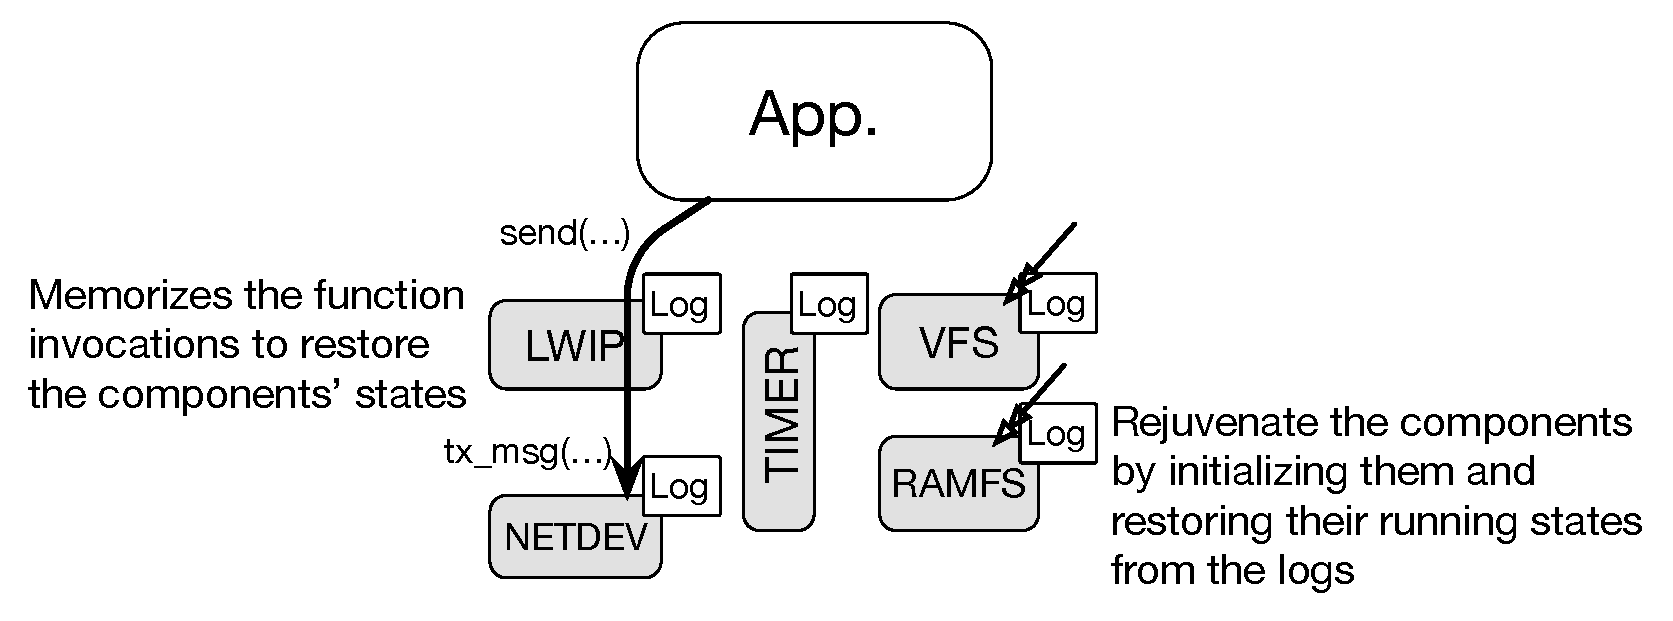
\includegraphics[scale=0.3]{./img/vampos.eps}
      \caption{\textbf{Overview of {\sysname}.} \textit{{\sysname} はコンポーネント単位での Unikernel の若返りを可能にする.そのために,\sysname は,各コンポーネントにより明確に定義され,公開されている関数をフックし,若返らせたコンポーネントの動作状態を復元するために関数呼び出しを記録する.}}
      \label{fig:overview}
    \end{center}
\end{figure}

これらの目標を達成するために,\sysname は Unikernel のカスタマイズ性を利用している.
Unikernel は多数のコンポーネントを提供し,
コンポーネント間のインタフェースが明確に定義されているため,
アプリケーションの動作に必要なコンポーネントのみを選択することができる.
\sysname の全体像を図\ref{fig:overview}に示す.
\sysname はコンポーネント単位での Unikernel の若返りを可能にし,
リンクしたアプリケーションを継続して実行できるように,
若返りしたコンポーネントの動作状態を復元する.
特に,\sysname は,公開されているコンポーネントインタフェースをフックすることにより,コンポーネント間のインタラクションを記録し,
ログを再生することで,状態を持つコンポーネントの動作状態を復元する.
例えば,ファイルシステムの若返りにおいては,\sysname は,
他のコンポーネントの動作状態の変更しないように,
そのコンポーネントのみを再起動し,若返りしたコンポーネント内部でログを再生する.

\sysname の目標は,\rr の効果を得ることであり,通常の再起動との完全な互換を目指しているものではない.
Unikernel を若返りのために,Unikernel がリンクしたアプリケーションの再起動の代わりに \sysname の再起動することができる.
\sysname のメカニズムは,
通常の再起動によるソフトウェアアップデートや再構成のような他の目的に適用するものではなく,
そのような目的のためには,通常の再起動が使われる.

\sysname の設計は以下の技術的な課題を提示する.
どのように,Unikernel をコンポーネント単位で若返らせるのか?
どのように,対象のコンポーネントのみを復元するのか?
どのように,若返りしたコンポーネントの状態を効率良く復元するのか?
次の章では,これらの課題に対する解決策を述べる.
以下の議論は Unikraft~\cite{KuenzerEtAl-Unikraft} 上のプロトタイプの開発に基づくものであるが,
IncludeOS~\cite{BratterudEtAl-IncludeOS} のような他の Unikernel にも十分に適用できる一般性を持つであろう.

\section{設計} \label{sec:design}


\sysname は,上記の設計上の課題に対するソフトウェアレベルの解決策を提供する.
コンポーネント単位で効率的に Unikernel を若返らせるために,
\sysname は各コンポーネントごとの専用のスレッドを用意し,
コンポーネントの若返りが
他のコンポーネントの実行に影響を与えるのを防ぐ.

関係のあるコンポーネントの動作状態に影響を与えるのを防ぐため,
\sysname は,ログの再生時に,再起動したコンポーネントをカプセル化する.
また,\sysname は,コンポーネント初期化後に取得したコンポーネントのメモリスナップショットを使用し,
選択的に対象のコンポーネントの状態を変化させる関数のみを実行します.


\subsection{マルチスレッド Unikernel コンポーネント}

Unikernel をコンポーネント単位で若返えらせるために,
Unikernel コンポーネントの実行について考慮する必要がある.
Unikernel は,ライブラリのように動作するため,
各コンポーネントはその機能を呼び出すスレッドコンテキストによって実行される.
Unikernel にリンクされたアプリケーションのスレッドがファイルを開くことを要求すると,
そのコンテキストは,ファイルシステム関連のコンポーネントを実行する.
本来のアプローチでは,スレッドコンテキストが対象のコンポーネントに到達したときに
そのコンポーネントを若返らせる.
この方法は,その実行に直接影響を与えるため,現在のコンテキストに関係ないコンポーネントを若返らせることができなくなる,
例えば,Unikernel にリンクされたアプリケーションがファイル関連の処理を実行している間は,
ネットワークコンポーネントを若返らせることができない.

この問題を解決するために,
\sysname はすべてのコンポーネントに専用のスレッドを割り当てて,
メッセージパッシング方式で相互に交流する.
この方式は,アプリケーションのコンテキストに対して, \sysname のコンポーネントの透過的な若返りを可能にする.
例えば,\sysname は,アプリケーションスレッドが使用していないコンポーネントを若返らせることができ,
若返りがアプリケーションの行動に影響を与えるのを防ぐ.
そして,再起動されたコンポーネントの動作状態を復元することで,
\sysname にリンクされたアプリケーションが再起動に渡って動作を継続し続けることができる.

\sysname のコンポーネントは,
それぞれ自身のデータ領域とヒープ領域を保持し,
自身に実装されている関数は,
呼び出し元コンポーネントのスレッドではなく,
自身に割り当てられている専用のスレッドによって実行される.
各スレッドは,
他のコンポーネントの関数の引数を呼び出し先のコンポーネントに渡すことにより,
その関数を呼び出し,関数の実行には,コンポーネントごとのデータ領域とヒープ領域が使われる.
通常の Unikernel では,アプリケーションがファイルを開くために,VFS (仮想ファイルシステム)のコンポーネントが公開する \textbf{open()} を呼び出す際には,
アプリケーションのスレッドコンテキストが VFS コンポーネントの \textbf{open()} へとジャンプする.
一方で, VampOS にリンクされたアプリケーションがファイルを開くには,
アプリケーションのスレッドが \textbf{open()} の引数を VFS コンポーネントに渡し,
VFS コンポーネントのスレッドが \textbf{open()} を実行する.
\sysname が引数を取り出するために,コンポーネントによって公開されたインタフェースをフックし,
呼び出し先のコンポーネントのメモリにその引数をコピーする.
関数の実行中に参照される引数は,
呼び出し元のコンポーネントのメモリにあるものではなく,
自身のメモリ上の複製されたものである.


\subsection{コンポーネントの若返り}

Unikernel のコンポーネント単位の若返りにおいて,
対象のコンポーネントの動作状態に注意を払う.
ファイルシステムやネットワークのような多くの OS サブシステムが状態を持ち,
それらの状態持つ Unikernel コンポーネントの再起動が
アプリケーションと他のコンポーネントが継続して動作させることができない.
例えば,ファイルオフセットを保持する VFS コンポーネントを若返りさせると,
ファイルオフセットが 0 に初期化されるため,
若返り後のアプリケーションのファイル操作を正しく行えなくなる.
ソフトウェア若化の観点から,
対象のコンポーネントのメモリスナップショットを再起動の直前に取得し,
動作状態を復元するのは意味がない.
なぜなら,
メモリリークやディスクリプタリーク,メモリフラグメンテーションを含む
古くなったメモリイメージが再作成されるからである.

\begin{figure}[t]
    \centering
    \includegraphics[width=\linewidth]{img/logging.pdf}
    \vspace{-5mm}
    \caption{コンポーネント間のインタラクションのロギング}
    \label{fig:logging}
\end{figure}

\begin{figure}[t]
    \centering
    \includegraphics[width=\linewidth]{img/playlog.pdf}
    \caption{コンポーネントの復元のためのログの再生}
    \label{fig:restoration}
\end{figure}

\rr を実現するために,\sysname のコンポーネントの若返りは,
ソフトウェア若化~\cite{HuangEtAl-rejuvenation,CotroneoEtAl-rejuvenation-survey,CotroneoEtAl-Surv14}のほかに,
クラッシュやハングアップからのリカバリにも使われる.
定期的にコンポーネントの若返りを行うことで,
コンポーネントの経年劣化による不具合を未然に防ぐことで,
Unikernel の動作を安定させる.
たとえ,クラッシュやハングアップが生じたとしても,
リアクティブにコンポーネントを若返らせることで,
Unikernel が動作を継続することができる,
クラッシュは CPU トラップ時のエラーコードによって検出でき,
ハングアップは関数実行に対してタイムアウトを設けることで検出する.


状態を持つコンポーネントの若返りによって生じる不整合を防ぐため,
再起動の後に状態を持つコンポーネントの動作状態を復元する.
復元のために,\sysname は,他のコンポーネントからの対象の関数に対する関数呼び出しを記録し,
若返りの後にコンポーネントのログを再生する.
図\ref{fig:logging}は,\sysname のコンポーネント間のインタラクションのロギングを表している.
他のコンポーネントに対して透過的に若返りしたコンポーネントの動作状態を復元するために,
{\sysname} はコンポーネントが公開するインタフェースをフックし,関数呼び出しを記録した後,値を返す.
若返り前に実行されたすべての関数を再実行するのではなく,
復元の時間の短縮およびメモリリークやメモリフラグメンテーションのような老化関連のバグによるエラー状態の再現を防ぐため,
\sysname は選択的に関数を呼び出す.
\sysname は,若返りの直前の状態を復元するのに必要な関数のみを呼び出す.
具体的には,ファイル状態の読み出し(\textbf{fstat()} 関連の関数)のようなコンポーネントの状態を変更しない関数は,
呼び出されない.
また,\sysname はすでに閉じられたファイルへの操作といった
コンポーネントの現在の状態を生成しない関数は再実行しない.

さらに,\sysname では,他のコンポーネントの関数を呼び出した際の戻り値のロギングも行う.
記録した関数の戻り値は,対象のコンポーネントの状態のみを復元するのに使われる.
ログの再生による関数の実行のための単純なアプローチは,
記録されている引数で,ただ,関数を実行することである.
しかし,このアプローチでは,
若返りしたコンポーネントの動作状態を復元している間に,
他のコンポーネントの関数を呼び出すことで,
そのコンポーネントの状態を変えてしまう.
これらの状態の変化は,通常の操作ではなく,復元の操作によって引き起こされるため,
動作中のアプリケーションと対応するコンポーネントとの不整合が生じる.
復元中に若返りしたコンポーネントから他のコンポーネントに状態を変化させる関数の呼び出しを防ぐために,
他のコンポーネントの関数を呼び出すのではなく,ログに記録された値を関数の戻り値として返す.
図\ref{fig:restoration}は,\sysname のコンポーネントの状態復元の概要である.
コンポーネントの若返りの後に,\sysname は自身の状態を復元するための関数をコンポーネントに実行させる.
その際,若返り前にログに記録した他のコンポーネントの関数呼び出しの戻り値を利用させることで,
その実行による他のコンポーネントの動作状態の変化を防ぐ.



\subsection{チェックポイントベースの若返り}

シャットダウンやブート処理を行う
通常のコンポーネントの再起動は,
コンポーネント単位の若返りには適していない.
その処理は,他のコンポーネントの関数呼び出しやハードウェアの操作を含み,
コンポーネントやハードウェアの動作状態を変化させてしまう.
例えば,RAM ファイルシステム上のメモリの読み書きを行う RAMFS コンポーネントは,
シャットダウンの段階でファイルシステム内のすべての内容を消去してしまう.

この問題を解決するために,
\sysname は,
phase-based reboot~\cite{YamakitaEtAl-PBR}のアイデアを借りて,
初期化直後のコンポーネントのメモリイメージを利用する.
この phase-based reboot では,起動段階でのシステムのメモリイメージを復元することによる
若返りの効果を獲得する.
\sysname は,コンポーネント単位のチェックポイントメカニズムを提供し,
初期化されたコンポーネントのメモリスナップショットを取得する.
前の章で述べたように,
コンポーネントの若返りにおいて,
\sysname はそのメモリスナップショットの復元とログの再生を実行する.


\subsection{Intel MPK を用いたエラー伝搬の防止}

コンポーネント間のエラー伝搬の防止には,
コンポーネントの粒度でのメモリの書き込み保護が必要である.
私たちは,コンポーネント単位での保護のために Intel の Memory Protection Keys (MPK)~\cite{Intel-MPK}
を使用する.
MPK は,CPU の命令セットアーキテクチャの拡張であり,
メモリのアクセス権限を細かい粒度で高速に制御することができる.
その有用性から,
MPK を用いたセキュリティメカニズム
がいくつか提案されている\cite{ParkEtAl-libmpk,HedayatiEtAl-Hodor,Schrammel-Donky,SartakovEtAl-ASPLOS21,LefeuvreEtAl-FlexOS}.
しかし,本研究は Unikernel の \rr をテーマとしており,
エラー伝搬防止のためだけに MPK を使用し,
Unikernel への攻撃を想定しない.


MPK では,ページ単位でメモリへの読み書きを制限できる.
各ページテーブルエントリ(PTE)には 4 ビットの保護キーが設定され,
CPU コアごとの PKRU レジスタには各保護キーの設定されたページへのアクセス権限が保存されている.
メモリアクセスの度に,
メモリ管理ユニット(MMU)が対象のページの保護キーで PKRU レジスタに保存されているアクセス権限を参照し,
権限がない場合にはページフォルトが発生する.

\sysname では,MPK の保護キーを各コンポーネントに割り当て,
コンポーネント外部からの書き込みを制限することで,
コンポーネント粒度でのメモリ保護を実現する.
コンポーネントスレッドは,自身の実行するコンポーネント以外のコンポーネントのデータへの書き込みができなくなり,
ほとんどのエラー伝搬を防ぐことができる.
このメカニズムで防ぐことができないエラー伝搬については,\ref{sec:disc}章で述べる.
あるコンポーネントスレッドが書き込み可能なコンポーネントは基本的に 1 つのみであるが,
コンポーネント間で関数引数の受け渡しを実現するために,
一時的に,別のコンポーネントの保護領域への書き込み権限が与えられることもある.


\section{評価実験} \label{sec:evaluation}


ソフトウェア若化を行う \sysname のプロトタイプを Unikraft 0.8.0 に実装し,実験を行った.
実験には,
Intel Xeon E5-2430 v2 (6 コア,2.5 GHz)と 16 GB の RAM を搭載する
PowerEdge T320 をハイパースレッディングを無効にして使用した.
本実験では,
ソフトウェア若化に関する基礎的な疑問である
\sysname に伴うオーバヘッドと
実アプリケーションおける \sysname の効果を確認することを目的とする.

\subsection{マイクロベンチマーク}

\begin{figure}[!t]
    \centering
    \includegraphics[width=\linewidth]{img/syscall-time.pdf}
    \caption{システムコールのオーバヘッド}
    \label{fig:func-time}
\end{figure}

\sysname によって生じるランタイムオーバヘッドを確認するために,
プロトタイプとデフォルトの Unikraft におけるシステムコールの実行時間を計測した.
特に,
\textbf{write()},\textbf{read()},\textbf{open()},\textbf{close()},\textbf{fstat()},\textbf{fcntl()} の 6 つのシステムコールの実行時間を計測した.
\textbf{write()},\textbf{read()} においては,
それぞれ,1 バイトのファイルに対して命令を発行している.
\textbf{open()},\textbf{close()} においては,
ファイルに対してただファイルディスクリプタを作成し,解放するという操作のみを行う.
\textbf{fstat()}では,ファイルの状態を取得し,
\textbf{fcntl()}では,ファイルディスクリプタのフラグを取得する.
\textbf{fcntl()}を除くこれらのシステムコール実行時には,VFS と RAMFS コンポーネント間のインタラクションが発生するのに対し,
\textbf{fcntl()}では,VFS コンポーネントのみを使用する.


実験の結果を
図\ref{fig:func-time}に示す.
図の横軸はシステムコールの種類を,
縦軸はその実行時間を表している.
図より,プロトタイプは最大で 13.60 倍のランタイムオーバヘッドを生じている.
このオーバヘッドは,デフォルトの Unikraft にはない \sysname におけるコンポーネントごとのスレッドのスケジューリングや
再起動後の動作状態を復元するための関数呼び出しのロギング,コンポーネントスレッド間のメッセージパッシング方式でのデータの受け渡し
によるものである.
また,
ランタイムオーバヘッドは元のシステムコールの実行時間が短いほど,
その倍率が大きくなる.
実際に,デフォルトの Unikraft と比較して,
\sysname の \textbf{read()} の実行時間が 6.38 倍であるのに対し,
\textbf{open()} の実行時間は 3.06 倍である.

\sysname の追加の処理にかかる時間は,
システムコールの種類に依存する.
\textbf{write()} のロギングにかかる時間が最も長いのは,
他のシステムコールよりも復元のためにより多くのデータを記録するためである.
一方で,
\textbf{open()} のデータ受け渡しにかかる時間が最も長いのは,
VFS と RAMFS コンポーネントが互いに実装された関数を呼び合い,
その実行のために追加のスレッドが生成されるためである.


\subsection{マクロベンチマーク}

\begin{figure}[!t]
    \centering
    \includegraphics[width=\linewidth]{img/SQLite-perf.pdf}
    \caption{SQLite のスループット}
    \label{fig:sqlite-perf}
\end{figure}

\begin{figure}[!t]
    \centering
    \includegraphics[width=\linewidth]{img/SQLite-mem.pdf}
    \caption{SQLite のメモリ消費量}
    \label{fig:sqlite-mem}
\end{figure}

実アプリケーションに対する \sysname の有効性を確認するために,
\sysname で SQLite を実行した.
SQLite は,汎用的なリレーショナルデータベース管理システム(RDBMS)であり,
Unikraft がサポートするアプリケーションの一つである.
本実験では,意図的にメモリリークのバグを挿入した \sysname で SQLite を起動し,
SELECT リクエストのスループットとメモリ消費量を計測する.
\sysname によるコンポーネントの再起動を行いながら,
SQLite を 30 分間動作させ続ける.
\sysname は,
VFS,RAMFS,スケジューラといった状態を持つ SQLite の Unikernel コンポーネントの再起動をラウンドロビン方式で行う.
\sysname は 30 秒ごとに一つずつコンポーネントの再起動を行う.
基準として,再起動を行わないデフォルトの Unikraft のスループットとメモリ消費量を計測する.
Unikraft の再起動は,RAM ファイルシステム上のデータベースの削除を伴い,
再起動を通して動作を継続できないため,
SQLite の再起動に使用することはできない.

図\ref{fig:sqlite-perf},\ref{fig:sqlite-mem} は,それぞれ,実験における SQLite のスループットとメモリ消費量を示している.
図\ref{fig:sqlite-perf} から,\sysname の再起動のための頻繁な再起動に対する長いダウンタイムを生じないことが分かる.
また,\sysname 上の SQLite のスループットは,デフォルトの Unikraft と同様に 30 秒ごとのコンポーネント単位の再起動をしながらも安定している.
しかし,前述したランタイムオーバヘッドにより,プロトタイプでのスループットがデフォルトの Unikraft の 半分程度になってしまう.
次の章では,実行時オーバーヘッドを軽減するために最適化が必要であることを述べる.


図\ref{fig:sqlite-mem} は,\sysname のプロトタイプがメモリリークを緩和していることを示している.
デフォルトの Unikraft のメモリ消費量は,
挿入したメモリリークのバグの影響で
線形に増加している.
一方,\sysname のログサイズが時間とともに増加するため,
プロトタイプのメモリ消費量は徐々に増加する.
\sysname のメモリオーバヘッドは,デフォルトの Unikraft のメモリ増加量よりも遥かに少ない.
今後,復元に不要なログを定期的に削除するなどのログのメモリ消費量を削減する仕組みを検討することが必要になる.

% \section{議論}
\label{sec:disc}

\subsection{エラー伝搬}

\sysname は Unikernel コンポーネントの高い強度での分離を
実現する CubicleOS~\cite{SartakovEtAl-ASPLOS21}や FlexOS~\cite{LefeuvreEtAl-FlexOS}と同じ強度で分離を実現するものであるものの,
このメカニズムで防ぐことができないエラー伝搬が存在する.
\sysname の分離メカニズムによって防ぐことができないエラー伝搬は,
関数呼び出し先のコンポーネントのエラーが関数呼び出し元のコンポーネントへと伝搬するケースである.
このケースは,正当な制御フローの範囲内にバグが存在するときに発生するものであり,
関数実行中のコンポーネントが呼び出し元のコンポーネントのデータを不当に更新することである.

このケースのエラー伝搬を完全に防ぐためには,
他のコンポーネントのデータ更新時の正当性を関数ごとに検証する必要がある.
しかし,Unikernel はアプリケーションの要件によって,コンポーネントの構成が異なるため,
同じ関数であっても,関数の呼び出し元と呼び出し先のコンポーネントの関係が一定であるとは限らず,
データ更新の正当性を定義することが難しい.



% \section{おわりに} \label{sec:conclusion}

\rr は,
定期的にメモリを若返らせたり,
クラッシュやハングアップからの
リアクティブなリカバリを行うことで,
コンピュータシステムの可用性や信頼性を向上させる.
新しいタイプの OS である Unikernel においても,
\rr は有効であるものの,
Unikernel レイヤのみの効率的な \rr の実現には,
いくつもの課題が存在する.
本論文では,それらの課題を明確にし,
解決するためのアプローチとして \sysname を紹介した.
最適化されていない \sysname のプロトタイプを用いた実験では,
ランタイムオーバヘッドに課題が残るものの,
ソフトウェア若化による経年劣化状態を解消することを確認した.



\bibliographystyle{ipsjunsrt}
\bibliography{paper}

\end{document}

